\chapter{Architettura del sistema}

\begin{figure}[htbp]
	\centering
	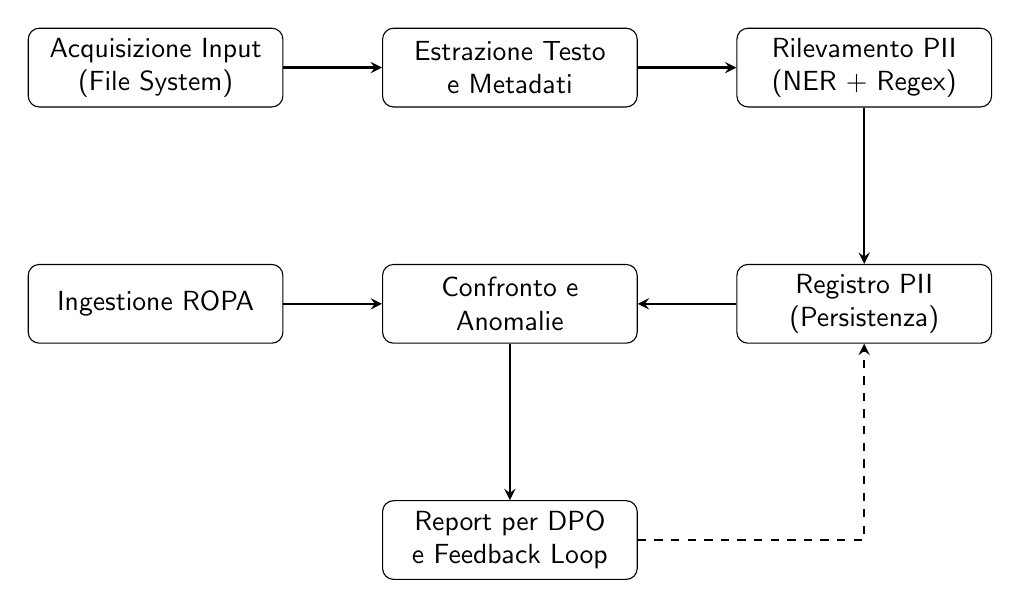
\begin{tikzpicture}[
			node distance=2cm,
			box/.style={rectangle, draw, rounded corners, minimum width=2.5cm, minimum height=1cm, text centered, font=\sffamily},
			arrow/.style={thick,->,>=stealth}
		]
		% Nodi
		\node[box, text width=3cm] (input) at (0, 0) {Acquisizione Input (File System)};
		\node[box, text width=3cm] (estrazione) at (4.5, 0) {Estrazione Testo e Metadati};
		\node[box, text width=3cm] (rilevamento) at (9, 0) {Rilevamento PII (NER + Regex)};

		\node[box, text width=3cm] (ropa) at (0, -3) {Ingestione ROPA};
		\node[box, text width=3cm] (confronto) at (4.5, -3) {Confronto e Anomalie};
		\node[box, text width=3cm] (registro) at (9, -3) {Registro PII (Persistenza)};

		\node[box, text width=3cm] (report) at (4.5, -6) {Report per DPO e Feedback Loop};

		% Frecce
		\draw[arrow] (input) -- (estrazione);
		\draw[arrow] (estrazione) -- (rilevamento);
		\draw[arrow] (rilevamento) -- (registro);

		\draw[arrow] (ropa) -- (confronto);
		\draw[arrow] (registro) -- (confronto);

		\draw[arrow] (confronto) -- (report);
		\draw[arrow, dashed] (report.east) -| (registro.south);
	\end{tikzpicture}
	\caption{Pipeline di esecuzione del sistema}
	\label{fig:architettura-pipeline}
\end{figure}

\begin{figure}[htbp]
	\centering
	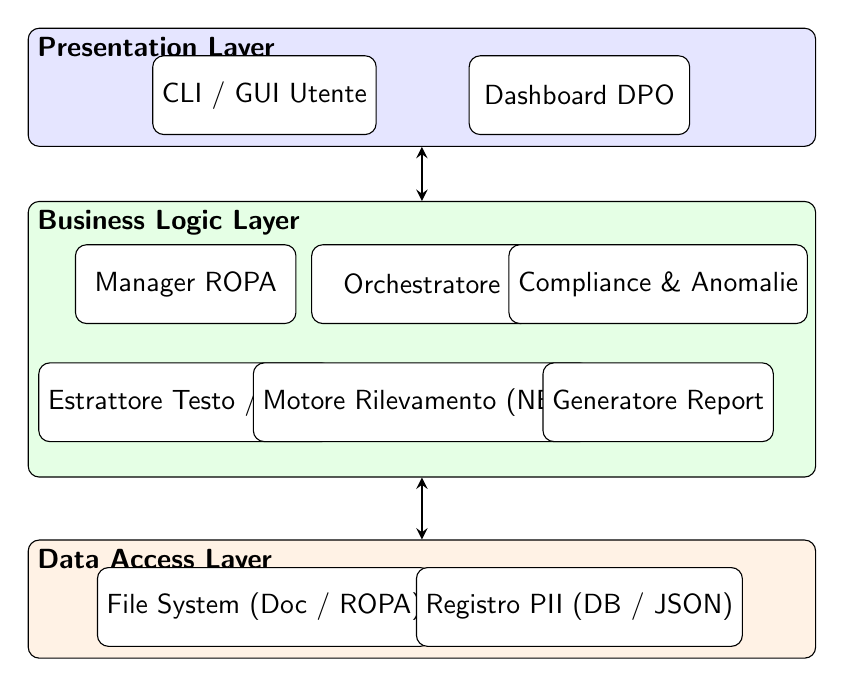
\begin{tikzpicture}[
			node distance=2cm,
			layer/.style={rectangle, draw, rounded corners, minimum width=10cm, minimum height=1.5cm, text centered, font=\sffamily, fill=gray!10},
			module/.style={rectangle, draw, rounded corners, minimum width=2.8cm, minimum height=1cm, text centered, font=\sffamily, fill=white},
			arrow/.style={thick,->,>=stealth}
		]

		% Livello Interfaccia
		\node[layer, fill=blue!10] (presentation) at (0, 0) {};
		\node[anchor=north west, font=\sffamily\bfseries] at (presentation.north west) {Presentation Layer};
		\node[module] (cli) at (-2, -0.1) {CLI / GUI Utente};
		\node[module] (dashboard) at (2, -0.1) {Dashboard DPO};

		% Livello Business Logic
		\node[layer, fill=green!10, minimum height=3.5cm] (logic) at (0, -3.2) {};
		\node[anchor=north west, font=\sffamily\bfseries] at (logic.north west) {Business Logic Layer};

		\node[module] (ropa_mgr) at (-3, -2.5) {Manager ROPA};
		\node[module] (orchestrator) at (0, -2.5) {Orchestratore};
		\node[module] (compliance) at (3, -2.5) {Compliance \& Anomalie};

		\node[module] (extractor) at (-3, -4) {Estrattore Testo / OCR};
		\node[module] (ner) at (0, -4) {Motore Rilevamento (NER)};
		\node[module] (report_gen) at (3, -4) {Generatore Report};

		% Livello Dati
		\node[layer, fill=orange!10] (data) at (0, -6.5) {};
		\node[anchor=north west, font=\sffamily\bfseries] at (data.north west) {Data Access Layer};
		\node[module] (fs) at (-2, -6.6) {File System (Doc / ROPA)};
		\node[module] (db) at (2, -6.6) {Registro PII (DB / JSON)};

		% Frecce / Relazioni tra livelli
		\draw[thick, <->, >=stealth] (presentation.south) -- (logic.north);
		\draw[thick, <->, >=stealth] (logic.south) -- (data.north);

	\end{tikzpicture}
	\caption{Suddivisione in moduli dell'architettura}
	\label{fig:architettura-moduli}
\end{figure}

\begin{figure}[htbp]
	\centering
	\begin{tikzpicture}[
			block/.style={rectangle, draw, rounded corners, minimum width=3.6cm,
					minimum height=1cm, align=center, fill=blue!8, font=\small},
			onetime/.style={rectangle, draw, dashed, rounded corners, minimum width=3.6cm,
					minimum height=1cm, align=center, fill=orange!10, font=\small},
			store/.style={cylinder, draw, shape border rotate=90, aspect=0.25,
					minimum height=1.6cm, minimum width=2.8cm, align=center, fill=gray!10, font=\small},
			input/.style={rectangle, draw, rounded corners, minimum width=3.2cm,
					minimum height=0.9cm, align=center, fill=green!8, font=\small},
			arrow/.style={thick, -{Latex[length=2mm]}},
		]

		% --- Input (riga y=0) ---
		\node (ropa) [input] at (0,0)   {ROPA\\(registro dei trattamenti)};
		\node (fs)   [input] at (6,0)   {File system\\/ documenti};

		% --- Blocchi una tantum (riga y=-2.4) ---
		\node (b1) [onetime] at (0,-2.4) {B1\\Normalizzazione ROPA\\(+ AI selettiva)};
		\node (b2) [onetime] at (6,-2.4) {B2\\Analisi struttura FS\\(+ AI selettiva, una tantum)};

		% --- Pipeline ricorrente (colonna destra, righe successive) ---
		\node (b3) [block] at (6,-4.8) {B3\\Estrazione \& normalizzazione\\testo (es. Docling)};
		\node (b4) [block] at (6,-7.2) {B4\\Pipeline ibrida detection\\(regex + NER + AI selettiva)};

		% --- Persistenza / associazione (riga y=-9.6) ---
		\node (b6) [block] at (0,-9.6) {B6\\Associazione\\documento--trattamento};
		\node (b5) [store] at (6,-9.6) {B5\\Registro PII\\rilevate};

		% --- Conformità e output ---
		\node (b7) [block] at (3,-12.0)  {B7\\Verifica conformità\\(retention, categorie, PII orfane)};
		\node (b8) [block] at (3,-14.4)  {B8\\Report / dashboard DPO};

		% --- Frecce: pipeline principale ---
		\draw [arrow] (ropa) -- (b1);
		\draw [arrow] (fs)   -- (b2);
		\draw [arrow] (b2)   -- (b3);
		\draw [arrow] (b3)   -- (b4);
		\draw [arrow] (b4)   -- (b5);
		\draw [arrow] (b5)   -- (b6);
		\draw [arrow] (b6)   -- (b7);
		\draw [arrow] (b7)   -- (b8);

		% --- Freccia B1 -> B6 (verticale, colonna libera) ---
		\draw [arrow] (b1) -- (b6);

		% --- Freccia B1 -> B7: corsia dedicata a sinistra, niente clipping ---
		\draw [arrow] (b1.west) -- ++(-1.2,0) |- (b7.west);

	\end{tikzpicture}
	\caption{Architettura a macro-blocchi del sistema (bozza)}
	\label{fig:architettura-macro-blocchi}
\end{figure}

\begin{figure}[htbp]
	\centering
	\begin{tikzpicture}[
			block/.style={rectangle, draw, rounded corners, minimum width=3.4cm,
					minimum height=1cm, align=center, fill=blue!8, font=\small},
			decision/.style={diamond, draw, minimum width=3cm, minimum height=1.2cm,
					align=center, fill=yellow!10, font=\small, aspect=2.2},
			ai/.style={rectangle, draw, dashed, rounded corners, minimum width=3.4cm,
					minimum height=1cm, align=center, fill=orange!10, font=\small},
			io/.style={rectangle, draw, rounded corners, minimum width=4cm,
					minimum height=0.9cm, align=center, fill=green!8, font=\small},
			arrow/.style={thick, -{Latex[length=2mm]}},
		]

		% --- Nodi ---
		\node (input)   [io]       at (0,    0)    {Testo normalizzato (da B3)};
		\node (regex)   [block]    at (-3.5, -2.5) {Regex\\(IBAN, CF, \ldots)};
		\node (ner)     [block]    at ( 3.5, -2.5) {NER\\(nomi, indirizzi, \ldots)};
		\node (merge)   [block]    at (0,    -5.2) {Merge risultati\\(overlap: sorgente doppia)};
		\node (counter) [decision] at (0,    -7.8) {ogni\\1000° doc?};
		\node (ai)      [ai]       at (6,    -7.8) {Passata AI\\(analisi contestuale)};
		\node (output)  [io]       at (0,   -10.5) {PII unificate $\rightarrow$ B5};

		% --- Fork: input -> regex + ner (parallelo) ---
		\coordinate (fk) at (0, -1.2);
		\draw [thick] (input.south) -- (fk);
		\draw [arrow] (fk) -| (regex.north);
		\draw [arrow] (fk) -| (ner.north);

		% --- Join: regex + ner -> merge ---
		\coordinate (jn) at (0, -4.2);
		\draw [thick] (regex.south) |- (jn);
		\draw [thick] (ner.south)   |- (jn);
		\draw [arrow] (jn) -- (merge.north);

		% --- Merge -> counter ---
		\draw [arrow] (merge.south) -- (counter.north);

		% --- Counter: No -> output ---
		\draw [arrow] (counter.south) -- node[right, font=\footnotesize]{No} (output.north);

		% --- Counter: Sì -> AI ---
		\draw [arrow] (counter.east) -- node[above, font=\footnotesize]{Sì} (ai.west);

		% --- AI -> output ---
		\draw [arrow] (ai.south) |- (output.east);

	\end{tikzpicture}
	\caption{Dettaglio del blocco B4: pipeline ibrida di rilevamento PII}
	\label{fig:b4-detection-pipeline}
\end{figure}

% TODO: INSERIRE QUI "CONFRONTO STRUTTURATO E SCELTA DEL MODELLO NER"
% Fare riferimento al file "Training_NER_confronto_strategie.md" (Sezione 3).
% Inserire la discussione e la tabella di confronto dei 3 approcci:
% A. Zero-shot puro (GLiNER base)
% B. Modello pre-fine-tunato da terzi (es. gliner-pii)
% C. Fine-tuning leggero in proprio
% Discutere perché, visti i vincoli e i requisiti del progetto (zero-training, no dati annotati, esecuzione locale), si scarta l'opzione C a favore delle opzioni A/B.
